% ============================================================ Capítulo 19
\chapter{Implementación del backend}\label{cap:backend}

\section{Estructura modular}
\begin{table}[H]\centering\small
\caption{Paquetes del backend}\label{tab:paquetes}
\begin{tabularx}{\linewidth}{@{}l X@{}}\toprule
Paquete & Contenido\\\midrule
\texttt{core} & Configuración (\texttt{pydantic-settings}), registro de eventos, jerarquía \texttt{ErrorFNA}.\\
\texttt{domain} & Modelos Pydantic (\texttt{RegistroCaptura}, \texttt{DocumentoLimpio}, \texttt{Fragmento},
\texttt{RespuestaQA}, \texttt{ResultadoFAQ}, \texttt{ResultadoResumen}\ldots) y puertos.\\
\texttt{knowledge} & \texttt{BaseConocimiento} (carga, búsqueda, filtros, contexto) e índice BM25.\\
\texttt{llm} & Catálogo de prompts YAML, cadenas LCEL, fábrica de proveedores, salvaguardas, modelo extractivo.\\
\texttt{repositories} & ORM y repositorio de auditoría (único acceso a SQL).\\
\texttt{services} & \texttt{ServicioAsistente} (fachada) y evaluación.\\
\texttt{api} & Aplicación FastAPI, DTO, dependencias inyectables y rutas.\\\bottomrule
\end{tabularx}
\end{table}

\section{Cadena LCEL de Q\&A}
\lstinputlisting[style=py,firstline=82,lastline=108]{../../src/fabrica_autopartes/llm/cadenas.py}

\section{Contratos de los endpoints}
\begin{longtable}{@{}P{1.1cm}P{4.3cm}P{4.4cm}P{5.4cm}@{}}
\caption{Contratos de entrada y salida}\label{tab:endpoints}\\\toprule
Método & Ruta & Entrada & Salida / errores\\\midrule\endfirsthead
\toprule Método & Ruta & Entrada & Salida / errores\\\midrule\endhead
GET & \texttt{/salud} & --- & \texttt{\{estado, version, fragmentos, proveedor\_llm, modelo\_llm\}}\\
GET & \texttt{/api/v1/base/estadisticas} & --- & \texttt{EstadisticasBase}\\
GET & \texttt{/api/v1/base/fragmentos} & \texttt{q}, \texttt{seccion}, \texttt{pagina}$\geq$1, \texttt{tamano} 1--100 &
\texttt{Pagina[FragmentoBuscado]} (con \texttt{puntaje} si hay \texttt{q})\\
GET & \texttt{/api/v1/base/fragmentos/\{id\}} & id con \texttt{\#} codificado como \texttt{\%23} & \texttt{Fragmento}; 404 \texttt{no\_encontrado}\\
POST & \texttt{/api/v1/tareas/qa} & \texttt{pregunta} (3--500), \texttt{proveedor}, \texttt{modelo}, \texttt{version\_prompt} (v1--v3),
\texttt{modo\_contexto} & \texttt{RespuestaQA}; 409 base vacía; 422 validación; 503 proveedor no disponible\\
POST & \texttt{/api/v1/tareas/faq} & \texttt{n\_preguntas} (3--20) + opciones LLM & \texttt{ResultadoFAQ}\\
POST & \texttt{/api/v1/tareas/resumen} & \texttt{enfoque} ($\leq$200) + opciones LLM & \texttt{ResultadoResumen}\\
GET & \texttt{/api/v1/auditoria/interacciones} & \texttt{pagina}, \texttt{tamano}, \texttt{tarea} & \texttt{Pagina[InteraccionDTO]}\\
GET & \texttt{/api/v1/pipeline/ejecuciones} & --- & \texttt{list[EjecucionDTO]}\\
POST & \texttt{/api/v1/pipeline/reconstruir} & cabecera \texttt{X-API-Key}; \texttt{fuente} & \texttt{EstadisticasBase}; 401 clave inválida; 403 sin clave configurada\\\bottomrule
\end{longtable}

\section{Manejo de errores, autenticación y auditoría}
Toda excepción de dominio hereda de \texttt{ErrorFNA} con \texttt{codigo} y \texttt{estado\_http}; un manejador
central devuelve \texttt{\{codigo, mensaje\}}. La operación administrativa compara la clave con
\texttt{secrets.compare\_digest} (tiempo constante) y queda deshabilitada si no hay clave configurada. CORS se
limita al origen de Streamlit. Cada tarea LLM se registra en \texttt{interacciones}.

\section{Verificación con Swagger y Postman}
\begin{lstlisting}[style=ps]
.\scripts\ejecutar_api.ps1                         # http://127.0.0.1:8000/docs (Swagger) y /redoc
Invoke-RestMethod http://127.0.0.1:8000/salud
$cuerpo = @{ pregunta = "¿Dónde queda la sede principal de Fanalca?"; version_prompt = "v3" } | ConvertTo-Json
Invoke-RestMethod -Method Post -Uri http://127.0.0.1:8000/api/v1/tareas/qa -ContentType "application/json; charset=utf-8" -Body $cuerpo
uv run fabrica openapi                             # exporta docs/api/openapi.json
\end{lstlisting}
La colección \ruta{postman/fabrica_autopartes.postman_collection.json} incluye 12 solicitudes en tres carpetas y
pruebas automáticas (estado 200, fundamentación, rechazo de dato ausente, bloqueo de inyección).

\begin{evidencia}[API ejecutada con uvicorn en el entorno de construcción (proveedor extractivo)]
\lstinputlisting[style=txt,firstline=3,lastline=4]{../evidencias/api_en_vivo.txt}
Swagger (\texttt{/docs}) respondió 200; \texttt{/api/v1/pipeline/reconstruir} sin clave respondió
\texttt{Operación deshabilitada: falta FNA\_API\_CLAVE\_ADMIN}; la pregunta de inyección quedó bloqueada.
Archivo completo: \ruta{docs/evidencias/api_en_vivo.txt}.
\end{evidencia}

% ============================================================ Capítulo 20
\chapter{Implementación del frontend}\label{cap:frontend}

\section{Justificación y vistas}
Streamlit (ADR-006) permite una interfaz funcional con poco código, adecuada para la demostración en vivo exigida.
La aplicación (\ruta{frontend/app.py}) invoca el servicio en proceso y se organiza en ocho pestañas.

\begin{table}[H]\centering\small
\caption{Vistas de la interfaz}\label{tab:vistas}
\begin{tabularx}{\linewidth}{@{}l X@{}}\toprule
Vista & Función\\\midrule
Panel & Métricas del corpus, fragmentos por sección, procedencia (URL) y últimas ejecuciones del pipeline.\\
Q\&A & Chat con botones de ejemplo; etiquetas de fundamentación, confianza, modo de contexto, modelo y latencia; fuentes enlazadas.\\
Resumen & Resumen ejecutivo con cuatro enfoques; descarga en Markdown.\\
FAQ & Preguntas frecuentes con fuentes por ítem y advertencias de ítems descartados; exportación CSV.\\
Laboratorio de prompts & Misma pregunta con v1, v2 y v3 lado a lado; muestra técnica, hipótesis y plantilla.\\
Evaluación & Ejecuta las 24 preguntas; métricas y detalle; histórico de evaluaciones.\\
Base de conocimiento & Búsqueda BM25 y filtro por sección; descarga del archivo consolidado; validación de calidad.\\
Auditoría & Interacciones registradas con filtro por tarea; exportación CSV.\\\bottomrule
\end{tabularx}
\end{table}
La barra lateral permite elegir proveedor, modelo, versión de prompt y modo de contexto. Un aviso visible indica
cuando la base proviene de la semilla. No se incluyen módulos ficticios: cada pestaña usa funciones del servicio
probadas.

\section{Asistente: fuentes, permisos y límites}
Fuente única: la base Gold. Permisos: solo lectura de la base y escritura de auditoría. Herramientas: ninguna
herramienta externa ni MCP durante la generación. Límites: preguntas de hasta 500 caracteres en la API, rechazo
explícito ante datos ausentes y bloqueo de inyección. Control contra respuestas no fundamentadas: verificación de
citas y fundamentación léxica, visibles como etiqueta en cada respuesta.

\section{Capturas}
\begin{figure}[H]\centering
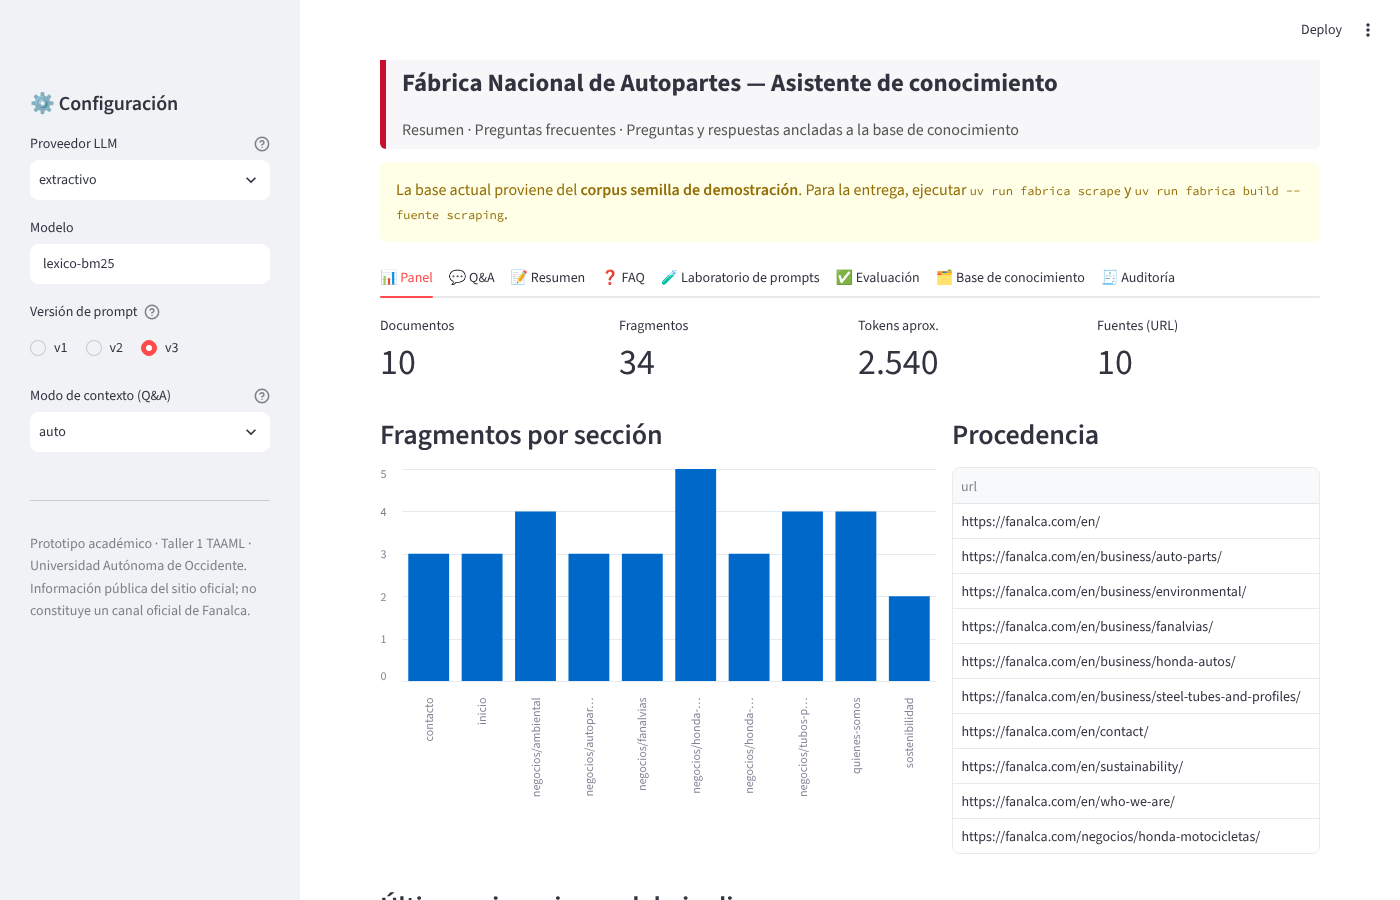
\includegraphics[width=0.92\linewidth]{figuras/ui_panel.png}
\caption{Panel con métricas del corpus y procedencia}\label{fig:ui-panel}
\end{figure}
\begin{figure}[H]\centering
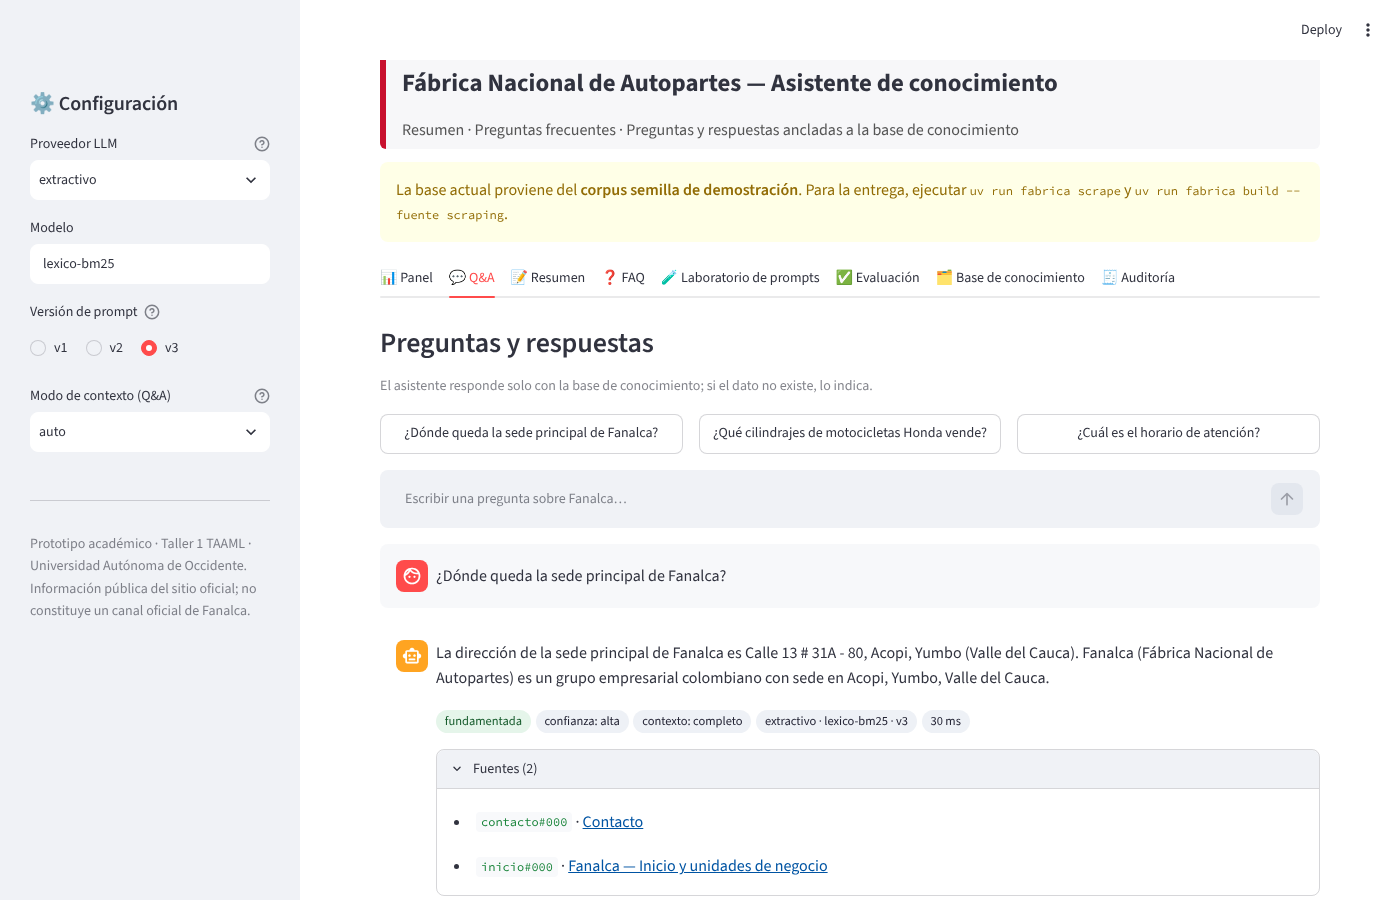
\includegraphics[width=0.92\linewidth]{figuras/ui_qa.png}
\caption{Q\&A con etiquetas de fundamentación y fuentes (proveedor extractivo)}\label{fig:ui-qa}
\end{figure}
\begin{figure}[H]\centering
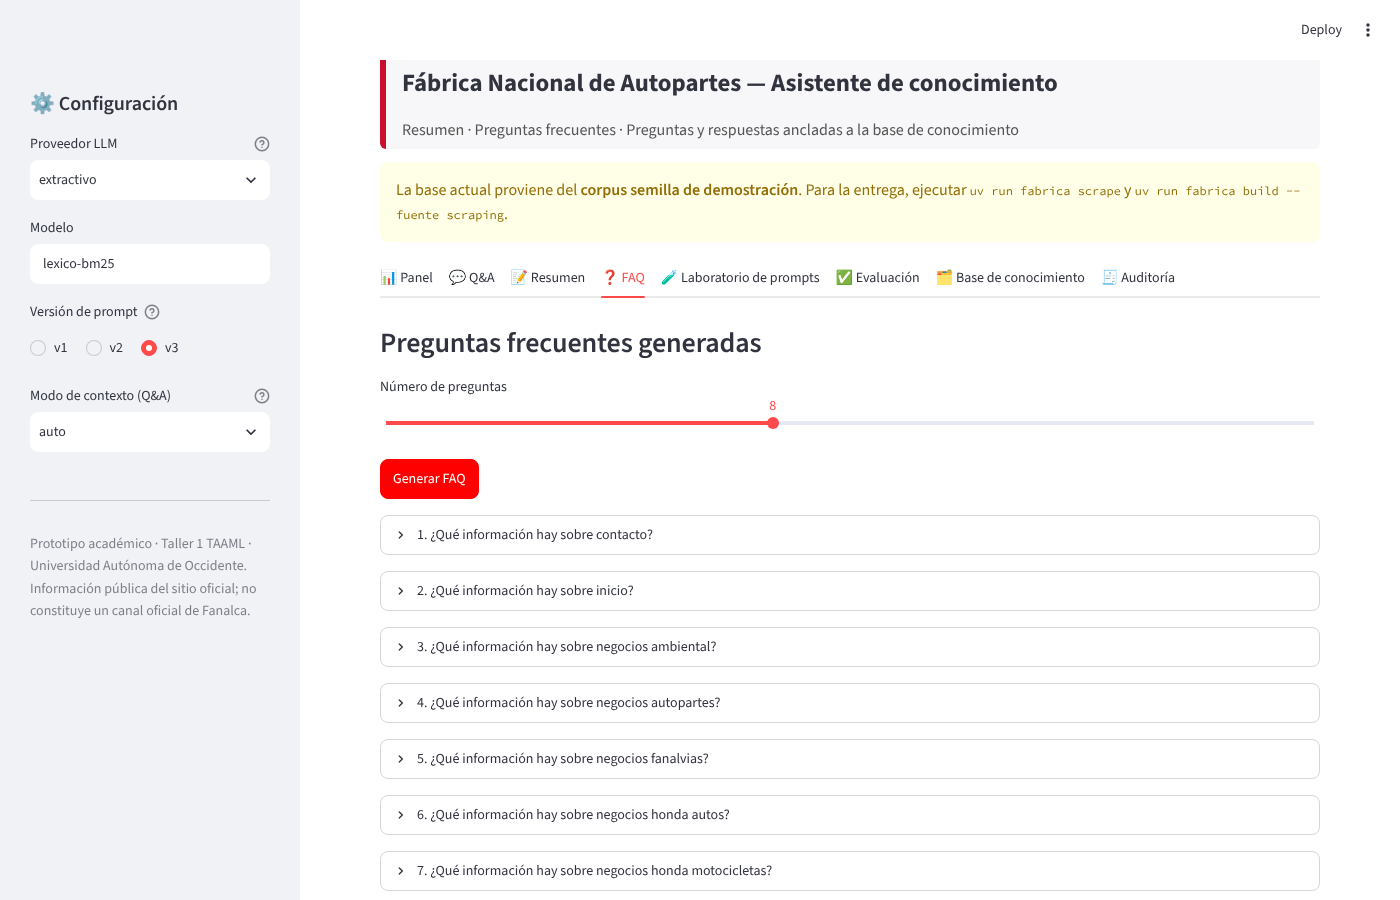
\includegraphics[width=0.92\linewidth]{figuras/ui_faq.png}
\caption{Generación de FAQ}\label{fig:ui-faq}
\end{figure}
\begin{figure}[H]\centering
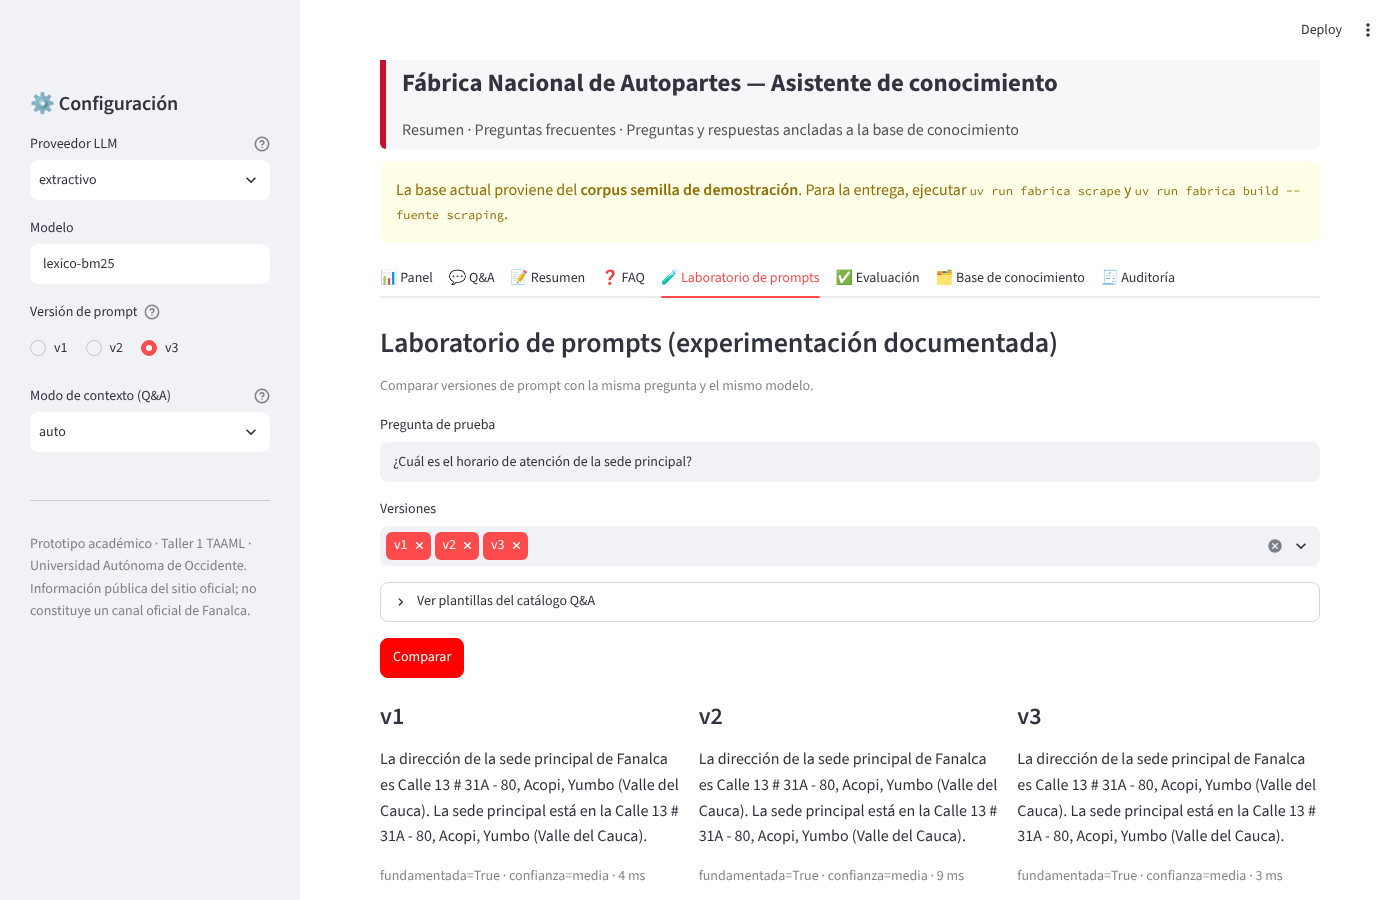
\includegraphics[width=0.92\linewidth,height=0.55\textheight,keepaspectratio]{figuras/ui_laboratorio.png}
\caption{Laboratorio de prompts: comparación de v1, v2 y v3}\label{fig:ui-lab}
\end{figure}
Las capturas se obtuvieron con Chrome sin interfaz sobre la aplicación en ejecución, con el proveedor
\texttt{extractivo}; con Ollama las respuestas son redactadas por el modelo.
